\section{Meat of the paper}

Here's the meat of the paper.

Figure~\ref{fig:picture} has a picture.

\begin{figure}[htbp]
\centerline{\resizebox{5in}{!}{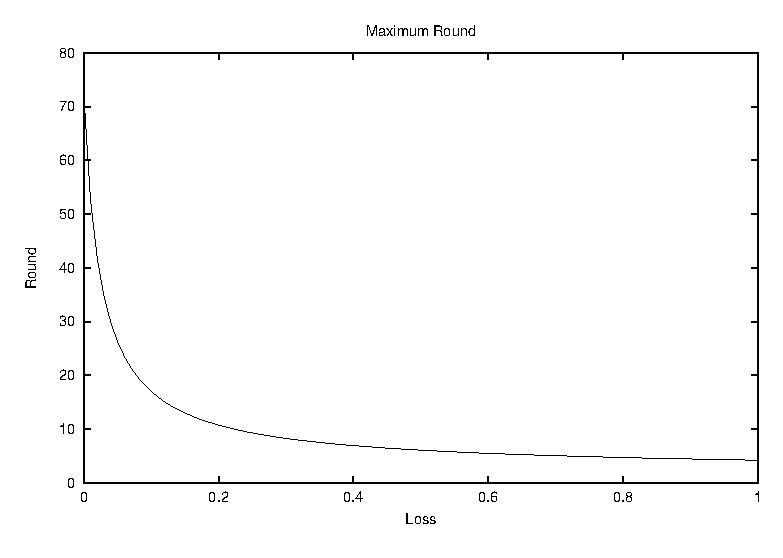
\includegraphics{maxround.ps}}}
\caption{\label{fig:picture} Picture of something that relates to Table~\ref{tab:mytable}}
\end{figure}

\noindent Here's the same picture but in another spot.
\begin{figure}[htbp]
\centerline{\resizebox{5in}{!}{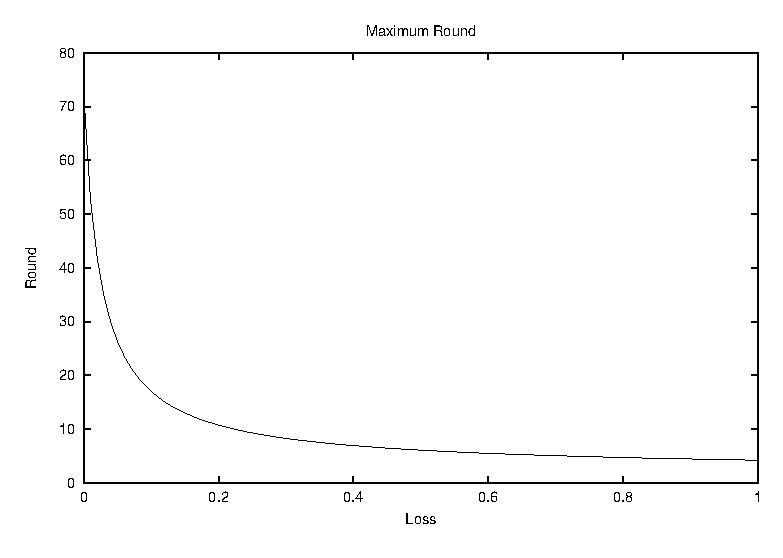
\includegraphics{maxround.ps}}}
\caption{\label{fig:repeatpicture} Repeat of Figure~\ref{fig:picture}}
\end{figure}

Here we use the macros

\[\summation{i=0}{N}{X^i}\]

\[\cond{X}{5}{if sky is blue}{6}{otherwise}\]
